\documentclass[a4paper,twoside]{report}

\usepackage{graphicx}
\usepackage{dsfont}

\usepackage{epsf,amsthm,amsmath}
\usepackage[ngerman]{babel}
\usepackage[latin1]{inputenc}
\usepackage{graphicx}
\setlength{\parskip}{5pt plus 8pt minus 2pt}
\pagestyle{headings}

%----------------------------------------------------------------------
%  Makros
%----------------------------------------------------------------------
%\usepackage{dsfont}
%\def\C{\mathds{C}}
%\def\F{\mathds{F}}
%\def\R{\mathds{R}}
%\def\N{\mathds{N}}
%\def\Z{\mathds{Z}}
%
%\newcommand{\bra}[1]{\langle#1|}
%\newcommand{\ket}[1]{|#1\rangle}
%\newcommand{\braket}[2]{\langle#1|#2\rangle}
%\newcommand{\ketbra}[2]{|#1\rangle\langle#2|}
%\newcommand{\projektor}[1]{|#1\rangle\langle#1|}
%\newcommand{\schnitt}[2]{
%   \raise3pt\vbox{\moveright6.5pt\hbox{$#1$}}\hspace*{-4pt}\Bigm/
%   \lower3pt\vbox{\moveleft6.5pt\hbox{$#2$}}}
%
%\newcommand{\includeeps}[2]{
%   \def\epsfsize##1##2{#2##1}
%   \centerline{\epsffile{#1}}}
%
%\newtheorem{satz}{Satz}[chapter]
%\newtheorem{bem}[satz]{Bemerkung}
%\newtheorem{lem}[satz]{Lemma}
%\newtheorem{defi}[satz]{Definition}
%\newtheorem{beispiel}[satz]{Beispiel}
%----------------------------------------------------------------------

\begin{document}
\begin{titlepage}
\ \vfill
\Large
\begin{center}
{\LARGE\bf Seminar} \\[1cm]
{\huge\bf Biologische Prinzipien in der Informatik\par}
\vspace*{1cm}
\input unilogo
\unilogo{30}\\[1cm]
{\bf Universit"at Karlsruhe (TH)}\\
{Fakult"at f"ur Informatik}\\
{\em Institut f"ur Prozessrechentechnik, Automation und Robotik}
\vfill
Prof. Dr. rer. nat. Brinkschulte\\
Manuel Nickschas\\
Florentin Picioroaga\\
Mathias Pacher\\
Sebastian Schuster\\
Alexander von Renteln	  
\vfill\vfill 
Sommersemester 2006
\vfill
\vfill
\end{center}
\end{titlepage} 
% 
%\newpage
%\thispagestyle{empty}
%\ 
%\newpage 
\thispagestyle{empty}
\ 
\vfill
\noindent
Copyright $\copyright$ 2006\\
Institut f"ur Prozessrechentechnik, Automation und Robotik (IPR)\\
Abteilung Prof. Dr. rer. nat. Brinkschulte (Mikrorechnertechnologien f"ur Automatisierung)\\
Geb"aude 40.28 - Engler-Bunte-Ring 8\\
76\,131 Karlsruhe
 
%\newpage 
%\thispagestyle{empty}
%\ 
%\newpage 



\title{Humorale Immunantwort}
\author{Clemens Lode}

\date{}
\maketitle

%\thispagestyle{empty}
%\newpage 

\pagenumbering{roman}
\tableofcontents

%\newpage 
\pagenumbering{arabic}


\setcounter{chapter}{0}
\chapter{Humorale Immunantwort}
\section{Einleitung}
In dieser Ausarbeitung geht es darum, wie ein System m"oglichst effektiv Fremdk"orper erkennen kann ohne von vornherein von deren Struktur zu wissen. Wichtige Punkte sind hier insbesondere die Unterscheidung von eigenen K"orperzellen und Fremdk"orpern wie auch das Verfahren wie sich das Immunsystem an die Umwelt anpassen kann, d.h. m"oglichst schnell m"oglichst viele Fremdk"orper erkennen kann.\\
\ \\
Auf biochemische und biophysikalische Details wurden aus Gr"unden des Umfangs nicht n"aher eingegangen, da sich die meisten Probleme in der Informatik nicht stellen. F"ur den zugrunde liegenden Algorithmus ist es irrelevant wie in der Realit"at z.B. zwischen den Zellen kommuniziert wird oder wie r"aumliche Strukturen erkannt werden.\\
\ \\
Desweiteren beschr"ankt sich diese Ausarbeitung auf die humorale Immunantwort, d.h. vor allem die Abl"aufe im Blut. Die mit der humoralen eng verbundenen zellul"are Immunantwort konzentriert sich auf die Abl"aufe in der (infizierten) Zelle und wird in einem anderen Vortrag besprochen.\\
\ \\
Prim"ares Augenmerk soll dabei eine Anwendung in der Informatik sein, die am Ende besprochen wird. Das Problem ein System vor Fremdk"orpern durch ein (Immun)System zu sch"utzen entspricht, neben den Details der biologischen Umsetzung, im Grunde dem Problem der Mustererkennung. Konkret ist es die Suche nach effizienten Schablonen die eine m"oglichst grosse Vielzahl an Fremdk"orpern erkennen, gleichzeitig aber nicht auf systemeigene Muster ansprechen. Die Anzahl der "Uberpr"ufungen und der Schablonen sind von Bedeutung, da sie sowohl den Speicheraufwand als auch die Rechengeschwindigkeit betreffen.

\newpage
\section{Grundeigenschaften des Immunsystems}


\subsection{Grunds"atzlicher Ablauf einer Immunantwort}

\begin{figure}[h]
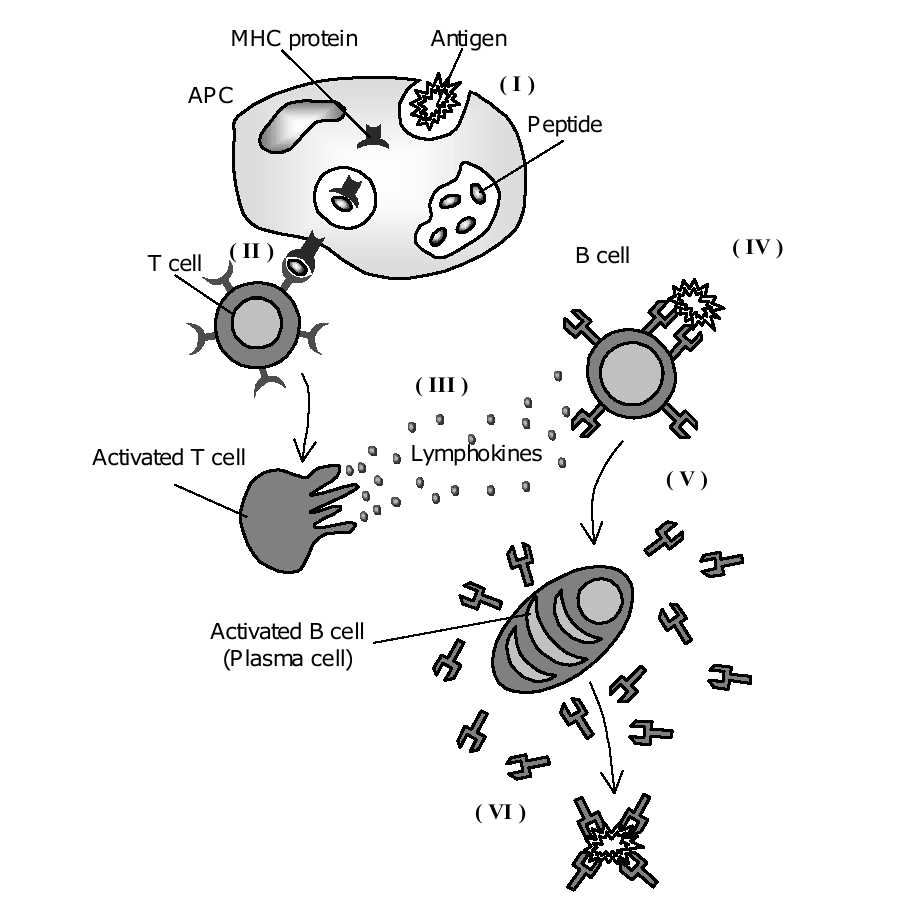
\includegraphics[scale=0.25]{immunablauf.png}
\caption{Ablauf einer Immunantwort}
\end{figure}

\begin{itemize}
\item Fresszellen, sogenannte Makrophagen, durchqueren den K"orper und nehmen die Oberfl"achenstrukturen, den sogenannten Antigenen, von Fremdk"orpern auf (I)
\item Aus den Antigenen werden sogenannte MHC-Molek"ule gebildet die auf der Oberfl"ache pr"asentiert werden (II)
\item Eine T-Zelle mit passendem Rezeptor f"ur das pr"asentierte MHC-Molek"ul kann nun an der Makrophage andocken und wird dadurch aktiviert
\item Die aktivierte Zelle sch"uttet Chemikalien, sogenannte Cytokine, aus, die wiederum B-Zellen aktivieren (III)
\item Die B-Zellen docken an Antigene bzw. antigenpr"asentierende Fremdk"orper an und werden zusammen mit den Cytookinen aktiviert (IV)
\item Die aktivierte B-Zelle teilt sich in Plasmazellen, die Antik"oper aussch"utten, und in langlebige Ged"achtniszellen als Schutz f"ur sp"atere Infektionen (V)
\item Die Antik"orper binden sich an die Antigene und markieren so die damit verbundenen Fremdk"orper (VI)
\end{itemize}

\subsection{Die sekund"are Immunantwort}

\begin{figure}[h]
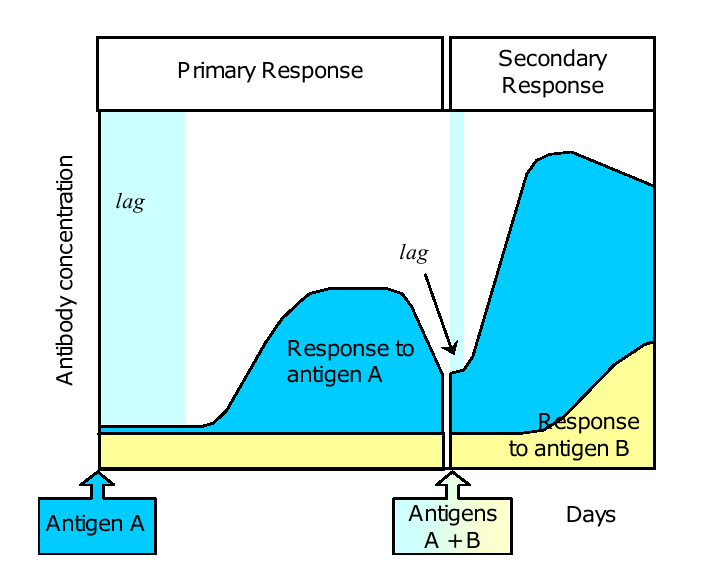
\includegraphics[scale=0.3]{immunsekundaer.png}
\caption{Prim"are und sekund"are Immunantwort}
\end{figure}

Wird das Immunsystem einmal mit unbekannten Antigenen konfrontiert, dann werden langlebige Ged"achtniszellen angelegt, die sich rasch vermehren, wenn sie erneut mit dem Antigen konfrontiert werden, meist aufgrund einer Infektion Tage bis Jahre nach der ersten Infektion. Diese sekund"are Immunantwort verl"auft wesentlich schneller und wesentlich effektiver als bei der ersten Immunantwort. Der Grund liegt darin, dass die Antik"orper auf diesen Typ von Fremdk"orper mit Hilfe von Mutation und Selektion st"arker spezialisiert sind als die Antik"orper die bei der ersten Immunantwort beteiligt waren. Somit k"onnen die Erreger fr"uher erkannt werden, was bei sich exponential vermehrenden Viren ein wesentlicher Vorteil ist.

\subsection{Impfung}
Neben dem nat"urlichen Weg einer Infektion (z.B. Tr"opfcheninfektion) besteht auch die M"oglichkeit das eigene Immunsystem mittels einer (Aktiv)Impfung mit der Krankheit zu konfrontieren. Dabei werden abgeschw"achte Erreger (inaktivierte Bakterientoxine oder Viren, abget"otete oder geschw"achte Bakterien oder auch isolierte Makromolek"ule bzw. deren Fragmente) gespritzt oder eingenommen. Dadurch kommt der K"orper mit den Fremdstoffen in Ber"uhrung, ist aber gleichzeitig nicht dem Risiko einer echten Krankheit ausgesetzt.\\
Demgegen"uber steht die Passivimpfung bei der nur die Antik"orper und nicht die Antigene injiziert werden.\\

\subsection{Aktive und passive Immunit"at}
Entsprechend r"uhrt die Unterscheidung zwischen aktiver und passiver Immunit"at von der Herkunft der Antik"orper im Blut. Aktive Immunit"at hat eine Person dann erworben, wenn das Immunsystem die Antik"orper selbst, als Antwort auf die Pr"asenz von Fremdstoffen, produziert hat. Dabei spielt es keine Rolle ob diese Pr"asenz nat"urliche Gr"unde hat oder k"unstlich mit z.B. einer Impfung herbeigef"uhrt wurde.\\
Passive Immunit"at bezeichnet den direkten "Ubergang von Antik"orpern entweder von einem Menschen auf den anderen (z.B. bei der Schwangerschaft, von der Mutter zum Kind) oder mit Hilfe einer Passivimpfung, bei der nur die Antik"orper und nicht die Antigene injiziert werden. Passive Immunit"at h"alt sich jedoch lediglich f"ur einige Wochen oder Monate, das k"orpereigene Immunsystem kennt die Antigene nicht und kann selbst auch keine eigenen Antik"orper dagegen produzieren, es kann eigene Abwehrkr"afte nur "uber einen direkten Kontakt mit Antigenen bilden.\\

\newpage
\section{Humorale Immunantwort}

\subsection{B-Zellen}
Bei Kontakt mit einem Fremdk"orper entwickelt sich ein Teil der B-Lymphozyten zu so genannten Plasmazellen, die Antik"orper gegen diesen Fremdk"orper bilden. Plasmazellen leben etwa 2-3 Tage. Aus dem anderen Teil der B-Lymphozyten werden nach Kontakt mit einem Fremdk"orper langlebige B-Ged"achtniszellen, die noch Jahre sp"ater, auch wenn der K"orper nicht mehr diesem Fremdk"orper ausgesetzt ist, die gleichen Antik"orper bilden k"onnen, was eine schnellere Reaktivierung der adaptiven Immunabwehr erm"oglicht.\\
Jede reife B-Zelle besitzt auf ihrer Oberfl"ache einen f"ur diese Zelle spezifischen Antik"orper, der als Antigenrezeptor fungiert und f"ur den diese Zelle f"ur den Rest ihres Lebens zust"andig ist. Die Antik"orper markieren Fremdk"orper und signalisieren dann anderen spezialisierten Zellen diese Fremdk"orper zu beseitigen.\\

\subsection{Aktivierung der T- und B-Zellen}
Der erste Schritt bei der Aktivierung der B-Zellen ist die Bindung eines Antigens an einen spezifischen Rezeptor auf der Oberfl"ache der B-Zelle. Um tats"achlich aktiv zu werden, gibt es im menschlichen Immunsystem aber noch einen Zwischenschritt um die Wahrscheinlichkeit fuer Autoimmunkrankheiten, d.h. die Erkennung eigener Zellen als Fremdk"orper, zu minimieren.\\
Makrophagen, die Fremdk"orper aufgenommen und verdaut haben, pr"asentieren dessen Antigene auf ihrer Oberfl"ache. T-Zellen erkennen diese Antigene durch Andocken an die Makrophage und klonen sich selbst zu einer spezialisierten T-Helferzelle die "uber Cytokine selektiv solche B-Zellen stimuliert, die mit einem solchen Antigen bereits zu tun gehabt haben.\\
B-Zellen pr"asentieren die Antigene auf ihrer Oberfl"ache und T-Zellen erkennen diese ebenfalls auf die selbe Weise. Der einzige Unterschied von Makrophagen und B-Zellen in dem Zusammenhang ist, dass Makrophagen mehrere verschiedene Antigene pr"asentieren k"onnen w"ahrend B-Zellen, wie auch T-Zellen, antigenspezifisch sind.\\
Sobald ein durch den Kontakt mit einer Makrophage und einer T-Zelle entstandene spezialisierter T-Helferzellenklon an das von der B-Zelle pr"asentierte Antigen angedockt hat, wird die B-Zelle aktiviert. Aktivierte B-Zellen differenzieren dann zu Plasmazellen und langlebigen Ged"achtniszellen.\\
Plasmazellen produzieren dann w"ahrend ihrer Lebenszeit Antik"orper bis die Infektion vor"uber ist und einige Tage dar"uber hinaus um eine Zweitinfektion rasch bek"ampfen zu k"onnen.


\subsection{Antigene und Antik"orper}

Als Antigen wird alles bezeichnet, was eine adaptive Immunreaktion ausl"osen kann. Die chemische Zusammensetzung ist dabei von geringer Bedeutung, Antik"orper erkennen Antigene nach ihrer dreidimensionalen Oberfl"achenstruktur. Oft hat ein Makromolek"ul mehrere solcher Strukturen, die unabh"agig voneinander die Bildung von Antik"orpern ausl"osen. Umgekehrt k"onnen zwei in der Prim"arstruktur ganz unterschiedliche Molek"ule trotzdem vom selben Antik"orper erkannt werden, wenn ihre Oberfl"achenstruktur zuf"allig sehr "ahnlich ist. Man spricht dann von einer Kreuzreaktion. T-Lymphozyten sind nicht auf dreidimensionale Epitope, sondern auf lineare Peptide von 8 bis 20 Aminos"auren L"ange spezialisiert.\\
Antik"orper verankern sich direkt mit den Antigenen, die sich auf der Oberflaeche des Fremdk"orpers befinden. Die so markierten Viren, auch "Antigen-Antikoerper-Komplex" genannt, werden dann durch phagocytotische Zellen beseitigt. Zus"atzlich k"onnen sich die Antik"orper zu Agglutinationen (Verklumpungen) zusammenschliessen, da jedes Antik"orpermolek"ul mindestens zwei Antigenbindungsstellen besitzt somit benachbarte Antigenmolek"ule vernetzen, den Fremdk"orper somit in seiner Funktion blockieren kann.

\subsection{Klonale Selektion}

\begin{figure}[h]
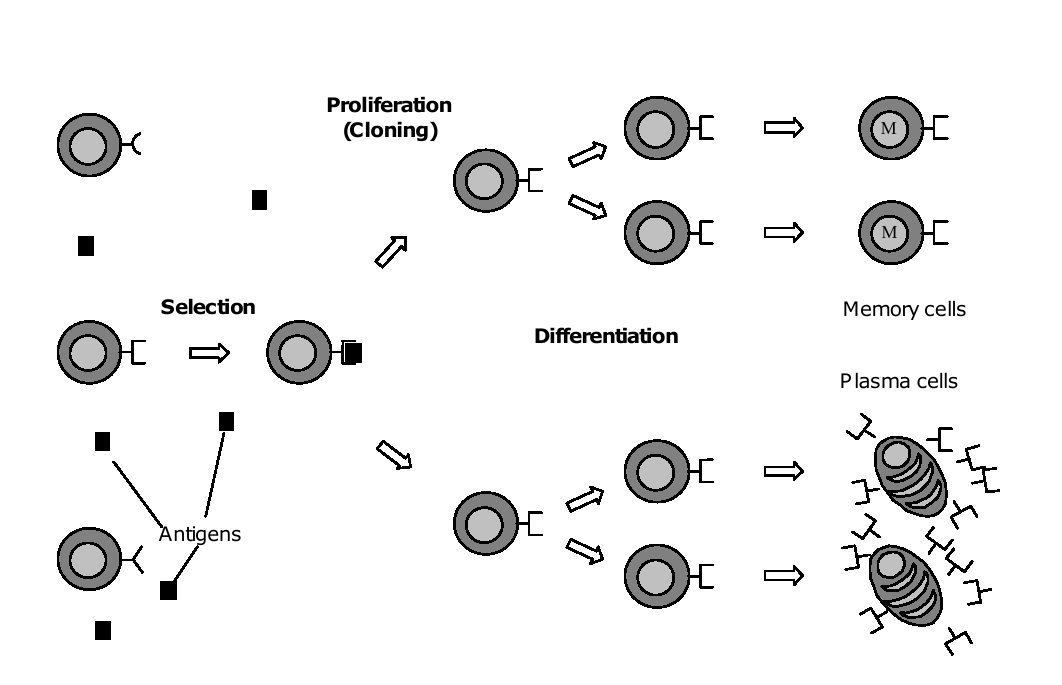
\includegraphics[scale=0.25]{immuncloning.png}
\caption{Klonale Selektion, B-Zellen mit hoher Antigenaffinit"at werden ausgew"ahlt}
\end{figure}

Die klonale Selektionstheorie stammt von F. McFarlane Burnet in den 50ger Jahren:\\
,,Einzelne Lymphozyten mit bestimmter Antigenspezifit"at sind in geringer Zahl vorhanden (pr"aexistieren) und werden aktiviert und vermehrt wenn das Antigen auftritt.''\\
\ \\
Jede Zellteilung/klonung ist mit Mutation und Rekombination der Gene verbunden, jede Lymphozyte hat somit eine individuelle Antigenspezifit"at. Nach der Infektion und Erkennung durch das Immunsystem werden besonders diejenigen T- und B-Zellen vermehrt, die eine hohe Antigenspezifit"at aufweisen, d.h. den Fremdk"orper besonders gut erkennen. Bei anderen T- und B-Zellen wird ein fr"uher Zelltod eingeleitet.\\
Zum Verst"andnis ist es entscheidend zu wissen, dass die sich im Blut befindlichen Immunzellen praktisch jeden Fremdk"orper erkennen k"onnen, die Immunantwort aber je nach Antigenspezifit"at unterschiedlich lange ben"otigt. Durch die klonale Selektion wird die Immunantwort lediglich optimiert. Dieser Mechanismus ist sehr "ahnlich der nat"urlichen Selektion in der Evolution und wird im letzten Kapitel etwas n"aher besprochen.\\
Der menschliche K"orper kann etwa \(10^{6}\) Proteine herstellen, das Immunsystem muss damit jedoch bis zu \(10^{16}\) Proteine bzw. Strukturen erkennen. Mittels Kombination genetisch vorliegender Gensequenzen k"onnen etwa \(10^{15}\) verschiedene Arten von Rezeptoren gebildet werden. Tats"achlich befinden sich aber nur etwa \(10^{8}\) bis \(10^{12}\) unterschiedliche Rezeptoren zu jedem Zeitpunkt im Immunsystem. Dieser Unterschied zwischen Zahl der zu erkennenden Strukturen und Zahl der Detektoren wird dadurch ausgeglichen, dass durch ungenaue Bindung an ein Antigen auch noch eine ganze Anzahl "ahnlicher Antigene erkannt werden k"onnen. Desweiteren werden durch die geringe Lebensdauer bedingte Neubildung der Lymphocyten immer wieder neue Muster gebildet.

\newpage

\section{Selbst-Fremd-Erkennung}

Um Fremdk"orper zu erkennen m"ussen nicht nur einfach Antigene erkannt werden, es muss auch festgestellt werden, ob es sich jeweils um ein k"orpereigenes oder ein k"orperfremdes Antigen handelt. Hierzu muss dem Immunsystem zum einen ein Merkmal vorliegen, das die eigenen Zellen eindeutig identifiziert und zum anderen muss dieses Merkmal gelernt werden. Das eindeutige Merkmal ist eine Gruppe von Proteinmolek"ulen die durch eine Anzahl von Genen codiert werden und ,,Haupthistokompatibilitaetskomplex'' (MHC-major histocompatibility complex) genannt werden. Aufgrund der grossen Anzahl von Kombinationsm"oglichkeiten (ca. 20 MHC-Gene und 100 Allele von jedem Gen) hat jeder Mensch einen unterschiedlichen MHC Marker.\\
Hierzu muss in kontrollierter Umgebung jede neuentstandene T-Zelle, die ja Schl"ussel in der Immunantwort ist, getestet werden, ob sie k"orpereigene Molek"ule erkennt und dann in dem Fall funktionsunf"ahig gemacht werden. Dieser Vorgang nennt sich ,,selektive Deletion'' und passiert im Thymus. In diesem Auswahlprozess werden etwa 95 Prozent aller neu gebildeten Zellen aussortiert, da sie k"orpereigene Strukturen erkennen. Funktioniert die Selektion nicht richtig, dann treten Autoimmunkrankheiten auf, das Immunsystem greift dann k"orpereigenes Gewebe an.\\
B-Zellen werden dezentral im Knochenmark gebildet, weshalb eine B-Zelle, um die Antik"orperproduktion anfangen zu k"onnen, sowohl mit dem Antigen an sich in Ber"uhrung kommen als auch ein Signal einer T-Zelle erhalten muss, die das Antigen ebenfalls erkannt hat. Da nur T-Zellen die Reifung im Thymus "uberstehen, die k"orperfremde Antigene erkennen, ben"otigt es deshalb keine weitere Sicherung f"ur die B-Zellen.
	
\section{Selbst-Fremd-Erkennung am Beispiel Bluttransfusion}
Blutzellen, wie jede K"orperzelle, haben spezifische Antigene auf ihrer Oberfl"ache. Im Menschen gibt es zwei verschiedene Antigene, A und B. Ein Mensch mit Blutgruppe A hat Blutzellen mit Antigen A und er besitzt Antik"orper zu Antigen B, ein Mensch mit Blutgruppe B hat Blutzellen mit Antigen B und besitzt Antik"orper zu Antigen A. Empf"angt ein Mensch mit Blutgruppe A Blut von einem Menschen mit Blutgruppe B werden diese Blutzellen als Fremdk"orper angesehen und vom Immunsystem angegriffen.\\
Sonderstellungen haben Menschen mit Blutgruppe 0, deren Blutzellen haben weder Antigene A oder B, sie k"onnen also jedem Menschen spenden. Umgekehrt haben sie aber Antik"orper gegen A und gegen B, k"onnen selbst also nur Blut von Menschen mit Blutgruppe 0 empfangen. Menschen mit Blutgruppe AB k"onnen selbst nur Menschen mit Blutgruppe AB spenden, da sie aber keine Antik"orper gegen A oder B haben, k"onnen sie Blut jeglichen Typs empfangen.\\
\ \\
Dass "uberhaupt Antik"orper gegen andere Blut-Antigene existieren, liegt daran, dass die Antigene recht einfach aufgebaut sind und auch bei einigen, ungef"ahrlichen Bakterien auftauchen. Beispielsweise in Menschen mit Blutgruppe A existieren keine Bakterien mit Antigen B, da sie vom Immunsystem unsch"adlich gemacht werden. Gleichzeitig erwirbt das Immunsystem dadurch auch eine Immunit"at gegen Blut mit Antigen B. Bakterien die Antigen A besitzen werden dagegen nicht angegriffen.\\
\ \\
Ein Sonderfall ist der sog. Rhesus-Faktor. Ein Embryo hat nicht die selben DNS wie die Mutter, es m"ussen also spezielle Vorkehrungen existieren, damit der Embryo nicht als Fremdk"orper abgestossen wird. Dies geschieht durch die Placenta-Barriere, die auch zur Versorgung des Kindes dient. Durch diese Barriere k"onnen Antik"orper der Klasse IgM nicht hindurch. Andere Antik"orper, gegen Blutzellen mit Antigenen gegen den Rhesus-Faktor der Blutzellen.\\
\ \\
Ist die Mutter selbst Rh-positiv, dann besitzt sie keine Antik"orper gegen den Rhesus-Faktor, kann auch keine bilden und es besteht kein Problem. Ist die Mutter selbst Rh-negativ kann es passieren, dass, wenn z.B. bei der Geburt kleine Blutmengen in den Kreislauf der Mutter gelangen, dort Antik"orper gegen den Rhesus-Faktor gebildet werden. Bei einer zweiten Schwangerschaft k"onnen diese gebildeten Antik"orper in den Organismus des Embryos gelangen und dort die Rh-positiven Blutzellen angreifen.\\
\ \\
Als Gegenmassnahme kann man der Mutter nach der Geburt durch eine Passivimpfung mit Anti-Rh-Antik"orpern injizieren. Dadurch bildet das m"utterliche Immunsystem keine eigenen Antik"orper und weitere Schwangerschaften sind m"oglich.

\newpage
\section{Umsetzung in der Informatik}

Im folgenden soll eine vereinfachte, auf die Grundprinzipien reduzierte Umsetzung des Immunalgorithmus in der Informatik dargestellt werden. Bei der Umsetzung in der Informatik sind einige die sich im menschlichen K"orper stellenden Probleme irrelevant, beispielsweise m"ussen nicht alle Funktionsbestandteile dezentralisiert sein wie im Immunsystem, der Algorithmus selbst muss nicht parallelisiert werden sondern kann zentral auf einer CPU ablaufen.

\subsection{Interne Darstellung}

Antik"orper und Antigene werden durch Bitstrings dargestellt. Trifft ein Antik"orper auf ein Antigen mit invertiertem Bitstring, dann wird das Antigen erkannt. Einzige Ausnahme ist, dass eine 0 sowohl auf eine 1 als auch auf eine 0 passt. Ein solches 'dontcare' Symbol ist, wie sp"ater klar wird, notwendig und ist auch im nat"urlichen Immunsystem verwirklicht. Eine 1 k"onnte man sich als r"aumliche Erhebung vorstellen, zwei 1en passen dann nicht auf einen Platz.

Es werden nun also solche Antik"orper-Bitstrings zuf"allig erstellt. Anschliessend wird gepr"uft, ob diese Bitstrings k"orpereigene Antigene erkennen (selektive Deletion, wie im Thymus). In der Anwendung in der Informatik hiesse das, dass dem kuenstlichen Immunsystem ein 'gesunder' Ablauf in einer Simulation vorgespielt wird und alle Antik"orper die auf diesen Ablauf ansprechen gel"oscht werden. Diese Bedingung muss erf"ullt sein, auch das menschliche Immunsystem wuerde nicht funktionieren, wenn die T-Zellen nicht aufgel"ost w"urden, die auf eigene Antigene ansprechen bzw. wenn im Thymus selbst Antigene von k"orperfremden und gef"ahrlichen Erregern liegen w"urden. W"urde eine T-Zelle alle Antigene erkennen, dann w"are das System zwar 'immun' gegen alle Fremdk"orper, erkennt sich aber auch selbst.\\
\ \\
Als n"achstes muss man sich Gedanken machen, wann ein Antik"orper ein Antigen erkennt. Wie gut ein Antik"orper auf ein Antigen passt, nennt man Antigenaffinit"at oder im Weiteren 'Fitness'. In diesem Zusammenhang benutzen wir folgende Formel f"ur die Fitness:\\
\ \\
Fitness ( Antik"orper a, Antigen g ) = Anzahl von 1-0 und 0-1 Kombinationen minus Anzahl von 1-1 Kombinationen\\
\ \\
Beispiel:\\
Antigen: 10111, Antik"orper1: 01101\\
2 gleiche bits, 3 ungleiche bits \(\Rightarrow\) Fitness: 1\\
Antigen: 10111, Antik"orper1: 01001\\
1 gleiche bits, 4 ungleiche bits \(\Rightarrow\) Fitness: 3\\
\ \\
Der Einfachheit halber sollen hier nur Bitstrings gleicher L"ange untersucht werden. Erlaubt man l"angere Antigenstrings ergeben sich zus"atzliche Effekte, insbesondere sprechen dann wahrscheinlich mehrere Antik"orper auf einen Fremdk"orper an. F"ur den Algorithmus selbst ist das aber nebens"achlich.\\
\ \\
Der Algorithmus basiert auf nat"urlicher Selektion. In einer Schleife wird die Qualit"at eines jeden Antik"orpers getestet, die besten L"osungen werden weiterverwendet und mutiert, die schlechtesten L"osungen werden verworfen. Wie Mutation und Selektion umgesetzt werden gibt es verschiedene Ans"atze (bei der Mutation z.B. Punktmutation, Verschiebung von Bl"ocken und bei der Selektion z.B. Prozentzahl der selektierten besten L"osungen, Wahrscheinlichkeitsverteilung f"ur die Weiterverwendung  usw.). Der Forschungsbereich der Evolution"aren Algorithmen besch"aftigt sich intensiv mit den Fragestellungen, wie all diese variablen Parameter und Optionen verwendet werden sollten um ein gutes Ergebnis zu bekommen.\\
Man l"asst nun also folgenden Algorithmus durchlaufen:\\
\ \\
{\raggedright
\\
Erstelle eine Anzahl n zuf"alliger Antik"orper ( n \(\ll\) \(2^{bitstringlaenge}\) )\\
\ \\
Schleife Beginn\\
\ \ Entferne Antik"orper die k"orpereigene Antigene erkennen\\
\ \ Pr"ufe die Fitness der Antik"orper bez"uglich der sich momentan im System befindlichen Antigene\\
\ \ W"ahle die Antik"orper mit der h"ochsten Fitness\\
\ \ L"osche die Antik"orper mit der geringsten Fitness\\
\ \ Klone die besten Antik"orper um wieder n Antik"orper im System zu haben\\
\ \ Mutiere die neuen Antik"orper\\
Schleife Ende\\
}
\ \\
\textbf{Beispiel}:\\
K"orperfremde Antigene: 1011, 1001, 0001\\
K"orpereigene Antigene: 0010, 1011\\
n = 4\\
\ \\
Antik"orper a1, a2, a3, a4: 0000, 1000, 0100, 1011\\
Fitness a1: 3 + 2 + 1 = 6\\
Fitness a2: 1 + 0 + 2 = 3\\
Fitness a3: - wird entfernt, erkennt k"orpereigenes Antigen\\
Fitness a4: -3 + -1 + 1 = -3\\
\ \\
a1 und a2 werden ausgew"ahlt und zuf"allig an einer Stelle mutiert:\\
neue Antik"orper: 0010, 0001, 1100, 1001\\
Fitness a1: 1 + 3 + 2 = 6\\
Fitness a2: 1 + 0 + -1 = 0\\
Fitness a3: 2 + 1 + 3 = 6\\
Fitness a4: -1 + -2 + 0 = -3\\
\ \\
a1 und a3 werden ausgew"ahlt und zuf"allig an einer Stelle mutiert:\\
neue Antik"orper: 0010, 0001, 1100, 1001\\
Fitness a1: 1 + 3 + 2 = 6\\
Fitness a2: 1 + 0 + -1 = 0\\
Fitness a3: 2 + 1 + 3 = 6\\
Fitness a4: -1 + -2 + 0 = -3\\

\newpage
\subsection{Code einer einfachen Umsetzung}

{\ttfamily \raggedright \scriptsize
#include <stdio.h>\\
#include <stdlib.h>\\
#include <time.h>\\
\\
#define LAENGE 10\\
#define ANTIKOERPER 4\\
#define FREMDE\underline ANTIGENE 10\\
#define EIGENE\underline ANTIGENE 2\\
#define WAEHLE\underline BESTE 2\\
#define DURCHLAEUFE 50\\
\ \\
void\ mutiere(int$\ast$\ array,\ int\ length)\\
\{\\
\ \ for(int\ i\ =\ 0;\ i\ <{}\ 10;\ i++)\\
\ \ \{\\
\ \ int\ punktmutation\ =\ rand()\%length;\\
\ \ int\ wert\ =\ array[punktmutation];\\
\ \ if(wert\ ==\ 0)\\
\ \ \ \ array[punktmutation]\ =\ 1;\\
\ \ else\ array[punktmutation]\ =\ 0;\\
\ \ \}\\
\}\\
\ \\
int\ fitness\underline\ funktion(int\ a,\ int\ b)\\
\{\\
\ \ if((a\ ==\ 0)\ \&\&\ (b\ ==\ 0))\\
\ \ \ \ return\ 0;\\
\ \ else\ if((a\ ==\ 1)\ \&\&\ (b\ ==\ 0))\\
\ \ \ \ return\ 1;\\
\ \ else\ if((a\ ==\ 0)\ \&\&\ (b\ ==\ 1))\\
\ \ \ \ return\ 1;\\
\ \ else\ if((a\ ==\ 1)\ \&\&\ (b\ ==\ 1))\\
\ \ \ \ return\ -{}1;\\
\}\\
\ \\
int\ main()\\
\{\\
\ \ srand(time(NULL));\\
\ \ int\ fremde\underline\ antigene[FREMDE\underline\ ANTIGENE][LAENGE];\\
\ \ int\ eigene\underline\ antigene[EIGENE\underline\ ANTIGENE][LAENGE];\\
\ \ int\ antikoerper[ANTIKOERPER][LAENGE];\\
\ \ int\ fitness[ANTIKOERPER];\\
\ \ int\ max\underline\ fitness[WAEHLE\underline\ BESTE];\\
\ \ int\ waehle\underline\ beste[WAEHLE\underline\ BESTE];\\
\ \ int\ ersetze[WAEHLE\underline\ BESTE];\\
\ \ int\ ersetze\underline\ zaehler;\\
\ \\
\ \ for(int\ j\ =\ 0;\ j\ <{}\ LAENGE;\ j++)\\
\ \ \{\\
\ \ \ \ for(int\ i\ =\ 0;\ i\ <{}\ ANTIKOERPER;\ i++)\\
\ \ \ \ \ \ antikoerper[i][j]\ =\ rand()\%2;\\
\ \ \ \ for(int\ i\ =\ 0;\ i\ <{}\ FREMDE\underline\ ANTIGENE;\ i++)\\
\ \ \ \ \ \ fremde\underline\ antigene[i][j]\ =\ rand()\%2;\\
\ \ \ \ for(int\ i\ =\ 0;\ i\ <{}\ EIGENE\underline\ ANTIGENE;\ i++)\\
\ \ \ \ \ \ eigene\underline\ antigene[i][j]\ =\ rand()\%2;\\
\ \ \}\\
\ \ for(int\ d\ =\ 0;\ d\ <{}\ DURCHLAEUFE;\ d++)\\
\ \ \{\\
\ \ \ \ for(int\ i\ =\ 0;\ i\ <{}\ ANTIKOERPER;\ i++)\\
\ \ \ \ \{\\
\ \ \ \ \ \ fitness[i]\ =\ 0;\\
\ \ \ \ \ \ for(int\ j\ =\ 0;\ j\ <{}\ FREMDE\underline\ ANTIGENE;\ j++)\\
\ \ \ \ \ \ \{\\
\ \ \ \ \ \ \ \ int\ summe\ =\ 0;\\
\ \ \ \ \ \ \ \ for(int\ k\ =\ 0;\ k\ <{}\ LAENGE;\ k++)\\
\ \ \ \ \ \ \ \ \ \ summe\ +=\ fitness\underline\ funktion(antikoerper[i][k],\ fremde\underline\ antigene[j][k]);\\
\ \ \ \ \ \ \ \ fitness[i]\ +=\ summe;\\
\ \ \ \ \ \ \}\\
\ \ \ \ \ \ bool\ erkennt\underline\ selbst\ =\ false;\\
\ \ \ \ \ \ for(int\ j\ =\ 0;\ j\ <{}\ EIGENE\underline\ ANTIGENE;\ j++)\\
\ \ \ \ \ \ \{\\
\ \ \ \ \ \ \ \ int\ n\ =\ 0;\\
\ \ \ \ \ \ \ \ for(int\ k\ =\ 0;\ k\ <{}\ LAENGE;\ k++)\\
\ \ \ \ \ \ \ \ \ \ n\ +=\ (fitness\underline\ funktion(antikoerper[i][k],\ eigene\underline\ antigene[j][k])\ ==\ -{}1)\ ?\ 1\ :\ 0;\\
\ \ \ \ \ \ \ \ if(n\ ==\ LAENGE)\\
\ \ \ \ \ \ \ \ \{\\
\ \ \ \ \ \ \ \ \ \ erkennt\underline\ selbst\ =\ true;\\
\ \ \ \ \ \ \ \ \ \ break;\\
\ \ \ \ \ \ \ \ \}\\
\ \ \ \ \ \ \}\\
\ \ \ \ \ \ if(erkennt\underline\ selbst)\\
\ \ \ \ \ \ \ \ fitness[i]\ =\ -{}9999;\\
\ \ \ \ \}\\
\ \\
\ \ \ \ for(int\ i\ =\ 0;\ i\ <{}\ WAEHLE\underline\ BESTE;\ i++)\\
\ \ \ \ \{\\
\ \ \ \ \ \ max\underline\ fitness[i]\ =\ fitness[i];\\
\ \ \ \ \ \ waehle\underline\ beste[i]\ =\ i;\\
\ \ \ \ \ \ ersetze[i]\ =\ i+WAEHLE\underline\ BESTE;\\
\ \ \ \ \}\\
\ \ \ \ for(int\ i\ =\ WAEHLE\underline\ BESTE;\ i\ <{}\ ANTIKOERPER;\ i++)\\
\ \ \ \ \{\\
\ \ \ \ \ \ bool\ schon\underline\ gewaehlt\ =\ false;\\
\ \ \ \ \ \ for(int\ j\ =\ 0;\ j\ <{}\ WAEHLE\underline\ BESTE;\ j++)\\
\ \ \ \ \ \ \ \ if(waehle\underline\ beste[j]\ ==\ i)\\
\ \ \ \ \ \ \ \ \{\\
\ \ \ \ \ \ \ \ \ \ schon\underline\ gewaehlt\ =\ true;\\
\ \ \ \ \ \ \ \ \ \ break;\\
\ \ \ \ \ \ \ \ \}\\
\ \ \ \ \ \ if(schon\underline\ gewaehlt)\\
\ \ \ \ \ \ \ \ continue;\\
\ \ \ \ \ \ int\ min\underline\ fitness\ =\ max\underline\ fitness[0];\\
\ \ \ \ \ \ int\ min\ =\ 0;\\
\ \ \ \ \ \ for(int\ j\ =\ 1;\ j\ <{}\ WAEHLE\underline\ BESTE;\ j++)\\
\ \ \ \ \ \ \ \ if(min\underline\ fitness\ >{}\ max\underline\ fitness[j])\\
\ \ \ \ \ \ \ \ \{\\
\ \ \ \ \ \ \ \ \ \ min\underline\ fitness\ =\ max\underline\ fitness[j];\\
\ \ \ \ \ \ \ \ \ \ min\ =\ j;\\
\ \ \ \ \ \ \ \ \}\\
\ \ \ \ \ \ \\
\ \ \ \ \ \ if(min\underline\ fitness\ <{}\ fitness[i])\\
\ \ \ \ \ \ \{\\
\ \ \ \ \ \ \ \ max\underline\ fitness[min]\ =\ fitness[i];\\
\ \ \ \ \ \ \ \ waehle\underline\ beste[min]\ =\ i;\\
\ \ \ \ \ \ \}\\
\ \ \ \ \}\\
\ \ \ \ ersetze\underline\ zaehler\ =\ 0;\\
\ \ \ \ for(int\ i\ =\ 0;\ i\ <{}\ ANTIKOERPER;\ i++)\\
\ \ \ \ \{\\
\ \ \ \ \ \ bool\ gewaehlt\ =\ false;\\
\ \ \ \ \ \ for(int\ j\ =\ 0;\ j\ <{}\ WAEHLE\underline\ BESTE;\ j++)\\
\ \ \ \ \ \ \ \ if(waehle\underline\ beste[j]\ ==\ i)\\
\ \ \ \ \ \ \ \ \{\\
\ \ \ \ \ \ \ \ \ \ gewaehlt\ =\ true;\\
\ \ \ \ \ \ \ \ \ \ break;\\
\ \ \ \ \ \ \ \ \}\\
\ \ \ \ \ \ if(!gewaehlt)\\
\ \ \ \ \ \ \{\\
\ \ \ \ \ \ \ \ ersetze[ersetze\underline\ zaehler]\ =\ i;\\
\ \ \ \ \ \ \ \ ersetze\underline\ zaehler++;\\
\ \ \ \ \ \ \}\\
\ \ \ \ \}\\
\ \\
\ \ \ \ for(int\ j\ =\ 0;\ j\ <{}\ WAEHLE\underline\ BESTE;\ j++)\\
\ \ \ \ \{\\
\ \ \ \ \ \ for(int\ k\ =\ 0;\ k\ <{}\ LAENGE;\ k++)\\
\ \ \ \ \ \ \ \ antikoerper[ersetze[j]][k]\ ==\ antikoerper[waehle\underline\ beste[j]][k];\\
\ \ \ \ \ \ mutiere(antikoerper[ersetze[j]],\ LAENGE);\\
\ \ \ \ \}\\
\ \ \}\\
\ \\
\ \ \\
\ \ return\ EXIT\underline\ SUCCESS;\\
\}\\
\ \\
\ \\
\}
\normalfont\normalsize

\newpage
\section{Anwendung in der Informatik}

Da der Immunalgorithmus im Kern nichts anderes als eine Spezialanwendung des evolution"aren Algorithmus ist, sind die Anwendungen nat"urlich vielf"altig. Es gibt allerdings einige Besonderheiten des Immunsystems die auch durchaus als Anwendung denkbar sind. Darunter ist Robotersteuerung, Optimierung, Sicherheit, Verteilte Agenten, Neuronale Netzwerke und nat"urlich Bild- und Mustererkennung. Sehr zu empfehlen ist das Paper von de Castro und Von Zuben, dort werden etwa 50 weitere m"ogliche Anwendungen besprochen, hier nur zwei weitere Beispiele:

\subsection{Virendetektion}

\begin{figure}[h]
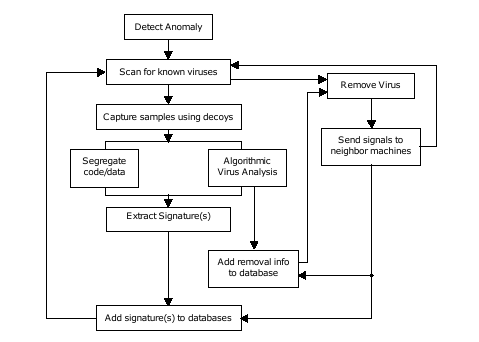
\includegraphics[scale=0.75]{immunvirus.png}
\caption{Klonale Selektion, B-Zellen mit hoher Antigenaffinit"at werden ausgew"ahlt}
\end{figure}

Das ist nat"urlich das erste was ins Auge springt. Die Software muss ,,eigene'', unsch"adliche Programme und b"osartige Programme unterscheiden und nutzt dabei aus, dass Virenprogramme meist bestimmtes Verhalten besitzen, wie z.B. sich resistent in den Speicher oder an bestimmten Positionen auf der Platte zu stellen. Checksums basieren auf der selben Idee. Desweiteren ist durch eine Anzahl von 'Decoy Programme' im Speicher die als ,,Beute'' f"ur ein Virus ausgelegt werden entspricht auch zu einem gewissen Teil des Prinzips der sich im Blut befindlichen Lymphocyten. Ausserdem ist das Warnen anderer Computersysteme eine effiziente Strategie die zentral und dezentral auch schon passiert (Sicherheitspatches, Newsgroups etc.).

\subsection{Netzwerkueberwachung}

Das Verhalten eines Netzflusses kann durch eine Vielzahl von Merkmalen kategorisiert werden, wie z.B. Geschwindigkeit, zugegriffene Ports oder IP-Adressen. Auch aus dem eigentlichen Datenfluss k"onnen stichprobenartig Signaturen entnommen werden.\\
Diese Informationen k"onnen in einen Bitstring als Antigen aufgefasst werden. Im k"unstlichen Thymus w"urde der Normallauf des Netzwerks simuliert werden wodurch dann ein k"unstliches Immunsystem verd"achtige "Anderungen im tats"achlichen Verlauf erkennen k"onnte.


\begin{thebibliography}{99}
\bibitem{Abk06} {\sc Neil A. Campbell}  \textit{Biologie}
\bibitem{wikipedia} \textit{wikipedia}
\bibitem{basic} {\sc Leandro Nunes de Castro, Fernando Jose Von Zuben 1999:} \textit{Artificial Immune Systems: Part I - Basic Theory and Applications}, ftp://ftp.dca.fee.unicamp.br/pub/docs/vonzuben/tr\underline\ dca/trdca0199.pdf
\bibitem{advanced} {\sc Leandro Nunes de Castro, Fernando Jose Von Zuben 2000:} \textit{Artificial Immune Systems: Part II - A Survey of Applications}, ftp://ftp.dca.fee.unicamp.br/pub/docs/vonzuben/tr\underline\ dca/trdca0200.pdf
\bibitem{overview} {\sc Steven A. Hofmeyr 1997:} \textit{An Overview of the Immune System}, http://www.cs.unm.edu/~immsec/html-imm/immune-system.html
\end{thebibliography}
\end{document}
